\documentclass[12pt]{extarticle}
\usepackage[english]{babel}
\usepackage{NotesTeX}
\usepackage{subfigure}
\usepackage{tikz}
\usetikzlibrary{arrows}
\usepackage{multirow}
\usepackage{listings}
\usepackage{extarrows}
\usepackage{parskip}
\usepackage{eurosym}
\usepackage{footmisc}

\collaborationImg{
\includegraphics[width=30mm]{../../pictures/UIO.png}}

\author{\Large Håkon Olav Torvik, Vetle Vikenes \& Sigurd Sørlie Rustad} 
\title{\Huge Project 2}
\affiliation{\large FYS-STK4155 – Applied Data Analysis and Machine Learning
\\Autumn 2021\\Department of Physics\\University of Oslo\\\\\today}
\begin{document}
\abstract{
	Abstract.
}
\maketitle

\section{Introduction}
\section{Theory}
In the theory-section we aim to give a brief explanation of the main concepts and terminology used in this report. For a more in-depth explanation we recommend reading the appropriate sections in \cite{2019}, which has been of great inspiration and help for us throughout the project.

\subsection{Gradient Decent}
In this section we cover gradient decent and different variations of it. More specifically we describe gradient decent (GD), stochastic gradient decent (SGD) and adding momentum to the aforementioned methods.
\subsubsection{Ordinary Gradient Decent}
Gradient decent methods is often used to minimize the so-called cost/loss-function. Thus, lets say we have a cost function $C(\boldsymbol{\beta})$ which could be expressed as
\begin{equation}
C(\boldsymbol{\beta}) = \sum_{i = 1}^{n}c_i(\mathbf{x}_i, \boldsymbol{\beta}).
\end{equation}
Where $n$ denotes the number of datapoints and $\mathbf x$ are the datapoints. The gradient with respect to the parameters $\boldsymbol{\beta}$ is then defined as
\begin{align}
\nabla_{\boldsymbol{\beta}} C(\boldsymbol{\beta}) = \sum_{i = 1}^{n} \nabla_{\boldsymbol{\beta}} c(\mathbf{x}_i, \boldsymbol{\beta}).
\label{eq:Total_gradient}
\end{align}
The algorithm for GD is then:
\begin{align}
\mathbf{v}_t &= \eta \nabla_{\boldsymbol{\beta}} C(\boldsymbol{\beta}_t) \nonumber \\
\boldsymbol{\beta}_{t+1} &= \boldsymbol{\beta}_t - \mathbf{v}_t,
\label{eq:GD_algo}
\end{align}
where $\eta$ is what we call the learning rate. This algorithms finds (ideally), with each iteration, new $\beta_{k+1}$ values which decreases the cost function. This is of course not always the case, and depends on the value of $\eta$. There are many potential problems when choosing the wrong learning rate. For example, if it is to big, our answer can diverge. If $\eta$ is too small we will need too many iterations to reach the minima, or reach a local minima.

\subsubsection{Stochastic Gradient Decent}
Another challenge, which is reduced when using SGD, are the large number of computations needed when calculating the gradient. Instead of calculating the total derivative as in \eqref{eq:Total_gradient}, we approximate it. This is done by performing the gradient on a subset of the data, called a minibatch. With $n$ still denoting the total number of datapoints, we will have $N_B=n/M$ minibatches, where $M$ is the size of each minibatch. The minibatches are denoted by $B_k$. Thus our approximated gradient, using a single minibatch $B_k$ is defined as
\begin{align}
\nabla_{\boldsymbol{\beta}} C^{MB}(\boldsymbol{\beta}) \equiv \sum_{i \in B_k} \nabla_{\boldsymbol{\beta}} c(\mathbf{x}_i, \boldsymbol{\beta}).
\end{align}
Then the aim is to use this approximated gradient, for all $N_B$ minibatches, to update the parameters $\boldsymbol{\beta}$, at every step $k$. Doing this for all $N_B$ minibatches, are what we refer to as an epoch. The SGD algorithm then becomes very similar to \eqref{eq:GD_algo}, however with an approximated gradient.
\begin{align}
\mathbf{v}_t &= \eta\nabla_{\boldsymbol{\beta}} C^{MB}(\boldsymbol{\beta}_t) \nonumber \\
\boldsymbol{\beta}_{t+1} &= \boldsymbol{\beta}_t - \mathbf{v}_t
\label{eq:SGD_algo}
\end{align}
This not only speeds up the algorithms, it also helps prevent getting stuck in local minima because of the stochastic nature.

\subsubsection{Adding Momentum}
Still the method can be optimized even further by adding momentum. This is done by a small modification in the parameter $\mathbf{v}_t$ in equations \eqref{eq:GD_algo} and \eqref{eq:SGD_algo}. Namely we add a so-called mass term, to simulate the step sizes having momentum
\begin{align}
	\mathbf{v}_t = \eta \nabla_{\boldsymbol{\beta}_t} C(\boldsymbol{\beta}) \rightarrow \mathbf{v}_t = \gamma \mathbf{v}_{t-1} + \eta \nabla_{\boldsymbol{\beta}} C(\boldsymbol{\beta}_t).
\end{align}
Here $\gamma$ is what we could refer to as the mass, and is another free parameter. One of the benefits is for example that this lets us move faster in regions where the gradient is small.

\subsection{Feed-Forward Deep Neural Networks}
Neural networks are neural-inspired nonlinear models, which are taught by a way of supervised learning. We will in this section explain what we mean by non-linearity, the basic architecture of a neural network and how the network learns. 
\subsubsection{Architecture of Neural Networks}
The structure we are going to use in this report is similar to that in figure \ref{fig:neural_network}. The gray circles are what we refer to as nodes. For now we just need to know that they hold some numerical value. One initializes the network by giving the nodes in the input layer numerical values. These values would correspond to some actual physical property, for example brightness of pixels in a picture. Then, each node in the input layer is connected to each node in the hidden layer $h_1$. In figure \ref{fig:neural_network} we have three such hidden layers, where each node in one layer is connected to every node in the next layer. Now the nodes are connected through what we will refer to as weights, biases and activation functions (more on that later). The connections are what assigns the numerical value of the nodes in the next layer. Lastly we have the output layer, which outputs values dependent on the problem. If we have a classification situation, where we for example wanted to classify the type of animal in different pictures, then one node could correspond to  a lion, next to a zebra and so fourth. By this we would know what animal the network \textit{thinks} is in the picture by looking at what neuron has the highest numerical value.

\begin{figure}[h]
	\minipage{0.70\textwidth}
	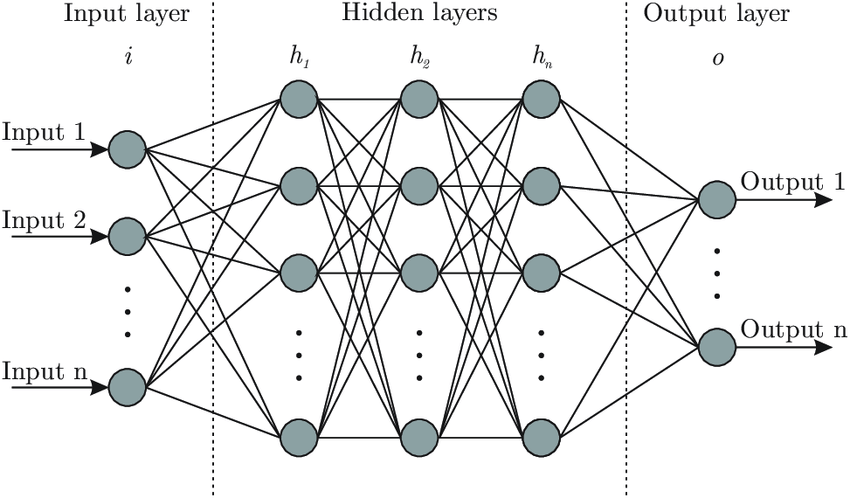
\includegraphics[width=\linewidth]{pictures/neural_network.png}
	(source: \texttt{https://www.researchgate.net/figure/Artificial-neur
		al-network-architecture-ANN-i-h-1-h-2-h-n-o\_fig1\_321259051})
	\endminipage\hfill
	\minipage{0.29\textwidth}
	\caption{Basic outline of a neural network. It displays the different layers (input, hidden and output), nodes (gray circles) and the connection between the nodes (black lines).}\label{fig:neural_network}
	\endminipage
\end{figure}

We mentioned that the different nodes are connected through weights, biases and activation functions. Looking at figure \ref{fig:neural_network}, a neuron $j$ in layer $h_1$ is connected to $n$ input neurons, denoted by black lines. Each input neuron has a numerical value defined by the problem. The value neuron $j$ in $h_1$ then gets is defined as
\begin{align}
\sigma (x_1w_1 + x_2w_2 + \dots + x_3w_n + b),
\end{align}
where $x_i$ are the values of neuron $i$ in the input layer, $w_i$ are the weights between neurons $i$ and $j$, $b$ is what we refer to as the bias and $\sigma$ is the activation functions (more on them in the next section). Every neuron is connected like this, with different weights and biases. In this project the activation function is the same for each neuron. Note that when we train the data, what we are really doing, is adjusting these parameters to give a desired result. We cover how this is done in the back propagation algorithm section.

\subsubsection{Activation Functions}
The activation functions are where the non-linearity term comes in, because they are non-linear. Now there are many such functions, in our project we have implemented the ones displayed in figure \ref{fig:activation_functions}. The exact functions are as follows
\begin{align}
	\text{Sigmoid: }\sigma(x) &= \frac{1}{1 + e^{-x}}\label{eq:sigmoid} \\
	\text{RELU: }\sigma(x) &= \max(0,x) \label{eq:RELU} \\
	\text{Leaky RELU: }\sigma(x) &= \begin{cases}
	\alpha x,& \text{if } x\leq 0 \\
	z,& \text{otherwise} 
	\end{cases} \label{eq:leaky_RELU}
\end{align}
Where $\alpha$ is some parameter which we have set to $\alpha = 0.1$ in figure \ref{fig:activation_functions}.

\begin{figure}[h]
	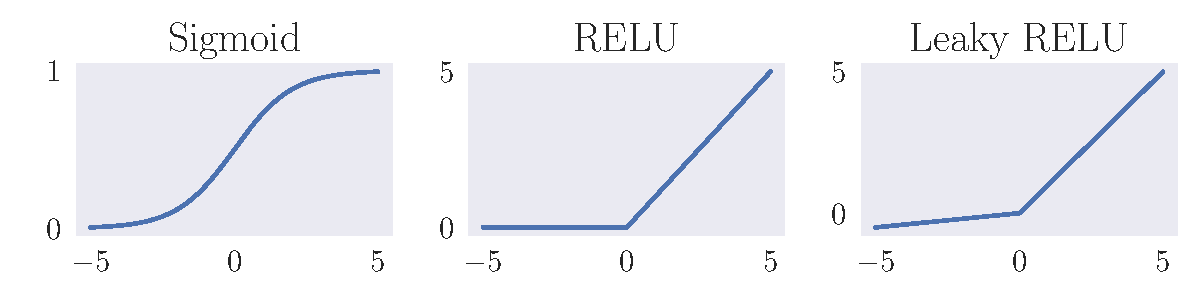
\includegraphics[width=\linewidth]{pictures/activation_functions.pdf}
	\caption{Some activation functions, namely Sigmoid, RELU and Leaky RELU.}\label{fig:activation_functions}
\end{figure}

\subsubsection{Cost Function and Regularization}
Before one can start training the data, we must have a cost function.
\subsubsection{The Back Propagation Algorithm}
\subsection{Logistic Regression}



\section{Methods}
\section{Results}
\section{Discussion}
\section{Conclusion}
\appendix
\section{Appendix}
\bibliographystyle{plain}
\bibliography{refs}
\end{document}

